%**************************************%
%*    Generated from PreTeXt source   *%
%*    on 2019-06-20T11:46:33-04:00    *%
%*                                    *%
%*   http://mathbook.pugetsound.edu   *%
%*                                    *%
%**************************************%
\documentclass[10pt,]{article}
%% Custom Preamble Entries, early (use latex.preamble.early)
%% Default LaTeX packages
%%   1.  always employed (or nearly so) for some purpose, or
%%   2.  a stylewriter may assume their presence
\usepackage{geometry}
%% Some aspects of the preamble are conditional,
%% the LaTeX engine is one such determinant
\usepackage{ifthen}
\usepackage{ifxetex,ifluatex}
%% Raster graphics inclusion
\usepackage{graphicx}
%% Colored boxes, and much more, though mostly styling
%% skins library provides "enhanced" skin, employing tikzpicture
%% boxes may be configured as "breakable" or "unbreakable"
%% "raster" controls grids of boxes, aka side-by-side
\usepackage{tcolorbox}
\tcbuselibrary{skins}
\tcbuselibrary{breakable}
\tcbuselibrary{raster}
%% xparse allows the construction of more robust commands,
%% this is a necessity for isolating styling and behavior
%% The tcolorbox library of the same name loads the base library
\tcbuselibrary{xparse}
%% Hyperref should be here, but likes to be loaded late
%%
%% Inline math delimiters, \(, \), need to be robust
%% 2016-01-31:  latexrelease.sty  supersedes  fixltx2e.sty
%% If  latexrelease.sty  exists, bugfix is in kernel
%% If not, bugfix is in  fixltx2e.sty
%% See:  https://tug.org/TUGboat/tb36-3/tb114ltnews22.pdf
%% and read "Fewer fragile commands" in distribution's  latexchanges.pdf
\IfFileExists{latexrelease.sty}{}{\usepackage{fixltx2e}}
%% Text height identically 9 inches, text width varies on point size
%% See Bringhurst 2.1.1 on measure for recommendations
%% 75 characters per line (count spaces, punctuation) is target
%% which is the upper limit of Bringhurst's recommendations
\geometry{letterpaper,total={340pt,9.0in}}
%% Custom Page Layout Adjustments (use latex.geometry)
%% This LaTeX file may be compiled with pdflatex, xelatex, or lualatex
%% The following provides engine-specific capabilities
%% Generally, xelatex and lualatex will do better languages other than US English
%% You can pick from the conditional if you will only ever use one engine
\ifthenelse{\boolean{xetex} \or \boolean{luatex}}{%
%% begin: xelatex and lualatex-specific configuration
%% fontspec package will make Latin Modern (lmodern) the default font
\ifxetex\usepackage{xltxtra}\fi
\usepackage{fontspec}
%% realscripts is the only part of xltxtra relevant to lualatex 
\ifluatex\usepackage{realscripts}\fi
%% 
%% Extensive support for other languages
\usepackage{polyglossia}
%% Main document language is US English
\setdefaultlanguage{english}
%% Spanish
\setotherlanguage{spanish}
%% Vietnamese
\setotherlanguage{vietnamese}
%% end: xelatex and lualatex-specific configuration
}{%
%% begin: pdflatex-specific configuration
%% translate common Unicode to their LaTeX equivalents
%% Also, fontenc with T1 makes CM-Super the default font
%% (\input{ix-utf8enc.dfu} from the "inputenx" package is possible addition (broken?)
\usepackage[T1]{fontenc}
\usepackage[utf8]{inputenc}
%% end: pdflatex-specific configuration
}
%% Monospace font: Inconsolata (zi4)
%% Sponsored by TUG: http://levien.com/type/myfonts/inconsolata.html
%% See package documentation for excellent instructions
%% One caveat, seem to need full file name to locate OTF files
%% Loads the "upquote" package as needed, so we don't have to
%% Upright quotes might come from the  textcomp  package, which we also use
%% We employ the shapely \ell to match Google Font version
%% pdflatex: "varqu" option produces best upright quotes
%% xelatex,lualatex: add StylisticSet 1 for shapely \ell
%% xelatex,lualatex: add StylisticSet 2 for plain zero
%% xelatex,lualatex: we add StylisticSet 3 for upright quotes
%% 
\ifthenelse{\boolean{xetex} \or \boolean{luatex}}{%
%% begin: xelatex and lualatex-specific monospace font
\usepackage{zi4}
\setmonofont[BoldFont=Inconsolatazi4-Bold.otf,StylisticSet={1,3}]{Inconsolatazi4-Regular.otf}
%% end: xelatex and lualatex-specific monospace font
}{%
%% begin: pdflatex-specific monospace font
%% "varqu" option provides textcomp \textquotedbl glyph
%% "varl"  option provides shapely "ell"
\usepackage[varqu,varl]{zi4}
%% end: pdflatex-specific monospace font
}
%% Symbols, align environment, bracket-matrix
\usepackage{amsmath}
\usepackage{amssymb}
%% allow page breaks within display mathematics anywhere
%% level 4 is maximally permissive
%% this is exactly the opposite of AMSmath package philosophy
%% there are per-display, and per-equation options to control this
%% split, aligned, gathered, and alignedat are not affected
\allowdisplaybreaks[4]
%% allow more columns to a matrix
%% can make this even bigger by overriding with  latex.preamble.late  processing option
\setcounter{MaxMatrixCols}{30}
%%
%% Color support, xcolor package
%% Always loaded, for: add/delete text, author tools
\PassOptionsToPackage{usenames,dvipsnames,svgnames,table}{xcolor}
\usepackage{xcolor}
%%
%% Semantic Macros
%% To preserve meaning in a LaTeX file
%% Only defined here if required in this document
%% Subdivision Numbering, Chapters, Sections, Subsections, etc
%% Subdivision numbers may be turned off at some level ("depth")
%% A section *always* has depth 1, contrary to us counting from the document root
%% The latex default is 3.  If a larger number is present here, then
%% removing this command may make some cross-references ambiguous
%% The precursor variable $numbering-maxlevel is checked for consistency in the common XSL file
\setcounter{secnumdepth}{3}
%% begin: General AMS environment setup
%% Environments built with amsthm package
\usepackage{amsthm}
%% Numbering for Theorems, Conjectures, Examples, Figures, etc
%% Controlled by  numbering.theorems.level  processing parameter
%% Numbering: all theorem-like numbered consecutively
%% i.e. Corollary 4.3 follows Theorem 4.2
%% Always need some theorem environment to set base numbering scheme
%% even if document has no theorems (but has other environments)
%% Create a never-used style first, always
%% simply to provide a global counter to use, namely "cthm"
\newtheorem{cthm}{BadTheoremStringName}[section]
%% end: General AMS environment setup
%% begin: environments with italicized bodies, theorems and similar
%% Style is like a theorem, and for statements without proofs
%% Theorem-like environments in modified "plain" style
%% We manage the head, do not adjust vertical spacing
%% Thus "space after theorem head" is necessary
%% This provides an automatic period after the number
\newtheoremstyle{ptxplainnotitle}
  {}% space above
  {}% space below
  {\itshape}% body font
  {}% indent amount
  {\bfseries}% theorem head font
  {.}% punctuation after theorem head
  {0.5em}% space after theorem head
  {}% theorem head specification
%% We now manage punctuation on-sight, elsewhere,
%% assuming non-trivial content inside a "title"
\newtheoremstyle{ptxplaintitle}
  {}% space above
  {}% space below
  {\itshape}% body font
  {}% indent amount
  {\bfseries}% theorem head font
  {}% punctuation after theorem head
  {0.5em}% space after theorem head
  {\thmname{#1}\thmnumber{ #2}\thmnote{ #3}}% theorem head specification
%% Only variants actually used in document appear here
%% Template eventually creates an environment of the given name
%% No arguments => Theorem 2.6. via "notitle" style variant
%% One optional argument => Theorem 2.6 Fantastic! via "title" style variant
%% AMS proof environment is basically fine as-is and special treatment
%% would certainly interfere with the functioning of \qed, etc.
%% So we simply localize the default heading
%% Redefinition of the "proof" environment is to cause a long alternate
%% title to line-break appropriately.  Code is cut verbatim, by suggestion,
%% from "Using the amsthm Package" Version 2.20.3, September 2017
%% end: environments with italicized bodies, theorems and similar
%% begin: environments with normal bodies, examples, etc.
%% Other environments go in modified "definition" style
%% Similar to above
\newtheoremstyle{ptxdefinitionnotitle}
  {}% space above
  {}% space below
  {}% body font
  {}% indent amount
  {\bfseries}% theorem head font
  {.}% punctuation after theorem head
  {0.5em}% space after theorem head
  {\thmname{#1}\thmnumber{ #2}}% theorem head specification
\newtheoremstyle{ptxdefinitiontitle}
  {}% space above
  {}% space below
  {}% body font
  {}% indent amount
  {\bfseries}% theorem head font
  {}% punctuation after theorem head
  {0.5em}% space after theorem head
  {\thmname{#1}\thmnumber{ #2}\thmnote{ #3}}% theorem head specification
%% end: environments with normal bodies, examples, etc.
%% Localize LaTeX supplied names (possibly none)
\renewcommand*{\abstractname}{Abstract}
%% Figures, Tables, Listings, Named Lists, Floats
%% The [H]ere option of the float package fixes floats in-place,
%% in deference to web usage, where floats are totally irrelevant
%% You can remove some of this setup, to restore standard LaTeX behavior
%% HOWEVER, numbering of figures/tables AND theorems/examples/remarks, etc
%% may de-synchronize with the numbering in the HTML version
%% You can remove the "placement={H}" option to allow flotation and
%% preserve numbering, BUT the numbering may then appear "out-of-order"
%% Floating environments: http://tex.stackexchange.com/questions/95631/
\usepackage{float}
\usepackage{newfloat}
\usepackage{caption}%% Adjust stock figure environment so that it no longer floats
\SetupFloatingEnvironment{figure}{fileext=lof,placement={H},within=section,name=Figure}
\captionsetup[figure]{labelfont=bf}
%% http://tex.stackexchange.com/questions/16195
\makeatletter
\let\c@figure\c@cthm
\makeatother
%% Program listing support: for listings, programs, and Sage code
\usepackage{listings}
%% We define the listings font style to be the default "ttfamily"
%% To fix hyphens/dashes rendered in PDF as fancy minus signs by listing
%% http://tex.stackexchange.com/questions/33185/listings-package-changes-hyphens-to-minus-signs
\makeatletter
\lst@CCPutMacro\lst@ProcessOther {"2D}{\lst@ttfamily{-{}}{-{}}}
\@empty\z@\@empty
\makeatother
\ifthenelse{\boolean{xetex}}{}{%
%% begin: pdflatex-specific listings configuration
%% translate U+0080 - U+00F0 to their textmode LaTeX equivalents
%% Data originally from https://www.w3.org/Math/characters/unicode.xml, 2016-07-23
%% Lines marked in XSL with "$" were converted from mathmode to textmode
\lstset{extendedchars=true}
\lstset{literate={ }{{~}}{1}{¡}{{\textexclamdown }}{1}{¢}{{\textcent }}{1}{£}{{\textsterling }}{1}{¤}{{\textcurrency }}{1}{¥}{{\textyen }}{1}{¦}{{\textbrokenbar }}{1}{§}{{\textsection }}{1}{¨}{{\textasciidieresis }}{1}{©}{{\textcopyright }}{1}{ª}{{\textordfeminine }}{1}{«}{{\guillemotleft }}{1}{¬}{{\textlnot }}{1}{­}{{\-}}{1}{®}{{\textregistered }}{1}{¯}{{\textasciimacron }}{1}{°}{{\textdegree }}{1}{±}{{\textpm }}{1}{²}{{\texttwosuperior }}{1}{³}{{\textthreesuperior }}{1}{´}{{\textasciiacute }}{1}{µ}{{\textmu }}{1}{¶}{{\textparagraph }}{1}{·}{{\textperiodcentered }}{1}{¸}{{\c{}}}{1}{¹}{{\textonesuperior }}{1}{º}{{\textordmasculine }}{1}{»}{{\guillemotright }}{1}{¼}{{\textonequarter }}{1}{½}{{\textonehalf }}{1}{¾}{{\textthreequarters }}{1}{¿}{{\textquestiondown }}{1}{À}{{\`{A}}}{1}{Á}{{\'{A}}}{1}{Â}{{\^{A}}}{1}{Ã}{{\~{A}}}{1}{Ä}{{\"{A}}}{1}{Å}{{\AA }}{1}{Æ}{{\AE }}{1}{Ç}{{\c{C}}}{1}{È}{{\`{E}}}{1}{É}{{\'{E}}}{1}{Ê}{{\^{E}}}{1}{Ë}{{\"{E}}}{1}{Ì}{{\`{I}}}{1}{Í}{{\'{I}}}{1}{Î}{{\^{I}}}{1}{Ï}{{\"{I}}}{1}{Ð}{{\DH }}{1}{Ñ}{{\~{N}}}{1}{Ò}{{\`{O}}}{1}{Ó}{{\'{O}}}{1}{Ô}{{\^{O}}}{1}{Õ}{{\~{O}}}{1}{Ö}{{\"{O}}}{1}{×}{{\texttimes }}{1}{Ø}{{\O }}{1}{Ù}{{\`{U}}}{1}{Ú}{{\'{U}}}{1}{Û}{{\^{U}}}{1}{Ü}{{\"{U}}}{1}{Ý}{{\'{Y}}}{1}{Þ}{{\TH }}{1}{ß}{{\ss }}{1}{à}{{\`{a}}}{1}{á}{{\'{a}}}{1}{â}{{\^{a}}}{1}{ã}{{\~{a}}}{1}{ä}{{\"{a}}}{1}{å}{{\aa }}{1}{æ}{{\ae }}{1}{ç}{{\c{c}}}{1}{è}{{\`{e}}}{1}{é}{{\'{e}}}{1}{ê}{{\^{e}}}{1}{ë}{{\"{e}}}{1}{ì}{{\`{\i}}}{1}{í}{{\'{\i}}}{1}{î}{{\^{\i}}}{1}{ï}{{\"{\i}}}{1}{ð}{{\dh }}{1}{ñ}{{\~{n}}}{1}{ò}{{\`{o}}}{1}{ó}{{\'{o}}}{1}{ô}{{\^{o}}}{1}{õ}{{\~{o}}}{1}{ö}{{\"{o}}}{1}{÷}{{\textdiv }}{1}{ø}{{\o }}{1}{ù}{{\`{u}}}{1}{ú}{{\'{u}}}{1}{û}{{\^{u}}}{1}{ü}{{\"{u}}}{1}{ý}{{\'{y}}}{1}{þ}{{\th }}{1}{ÿ}{{\"{y}}}{1}}
%% end: pdflatex-specific listings configuration
}
%% End of generic listing adjustments
%% Sage's blue is 50%, we go way lighter (blue!05 would work)
\definecolor{sageblue}{rgb}{0.95,0.95,1}
%% Sage input, listings package: Python syntax, boxed, colored, line breaking
%% To be flush with surrounding text's margins, set
%% xmargins to be sum of framerule, framesep, and epsilon (~0.25pt)
%% space between input/output comes from input style "belowskip",
%% by giving output an aboveskip of zero
\lstdefinestyle{sageinputstyle}{language=Python,breaklines=true,breakatwhitespace=true,%
basicstyle=\small\ttfamily,columns=fixed,frame=single,backgroundcolor=\color{sageblue},%
framerule=0.5pt,framesep=4pt,xleftmargin=4.75pt,xrightmargin=4.75pt}
%% Sage output, similar, but not boxed, not colored
\lstdefinestyle{sageoutputstyle}{language=Python,breaklines=true,%
breakatwhitespace=true,basicstyle=\small\ttfamily,columns=fixed,aboveskip=0pt}
%% The environments manufactured by the listings package
\lstnewenvironment{sageinput}
  {\lstset{style=sageinputstyle}}
  {}
\lstnewenvironment{sageoutput}
  {\lstset{style=sageoutputstyle}}
  {}
%% More flexible list management, esp. for references
%% But also for specifying labels (i.e. custom order) on nested lists
\usepackage{enumitem}
%% hyperref driver does not need to be specified, it will be detected
\usepackage{hyperref}
%% configure hyperref's  \url  to match listings' inline verbatim
\renewcommand\UrlFont{\small\ttfamily}
%% Hyperlinking active in PDFs, all links solid and blue
\hypersetup{colorlinks=true,linkcolor=blue,citecolor=blue,filecolor=blue,urlcolor=blue}
\hypersetup{pdftitle={UTMOST Instructors Guide}}
%% If you manually remove hyperref, leave in this next command
\providecommand\phantomsection{}
%% If tikz has been loaded, replace ampersand with \amp macro
%% tcolorbox styles for sidebyside layout
\tcbset{ sbsstyle/.style={raster equal height=rows,raster force size=false} }
\tcbset{ sbsheadingstyle/.style={size=minimal,halign=center,fontupper=\bfseries,colback=white,frame empty} }
\tcbset{ sbspanelstyle/.style={size=minimal,colback=white,frame empty} }
\tcbset{ sbscaptionstyle/.style={size=minimal,halign=center,colback=white,frame empty} }
%% Enviroments for side-by-side and components
%% Necessary to use \NewTColorBox for boxes of the panels
%% "newfloat" environment to squash page-breaks within a single sidebyside
%% \leavevmode necessary when a side-by-side comes first, right after a heading
\DeclareFloatingEnvironment[placement={H}]{sbscontainer}
%% "xparse" environment for entire sidebyside
\NewDocumentEnvironment{sidebyside}{mmmm}
  {\begin{sbscontainer}\begin{tcbraster}
    [sbsstyle,raster columns=#1,
    raster left skip=#2\linewidth,raster right skip=#3\linewidth,raster column skip=#4\linewidth]}
  {\end{tcbraster}\end{sbscontainer}}
%% "tcolorbox" environments for three components of a panel
\NewTColorBox{sbsheading}{m}{sbsheadingstyle,width=#1\linewidth}
\NewTColorBox{sbspanel}{mO{top}}{sbspanelstyle,width=#1\linewidth,valign=#2}
\NewTColorBox{sbscaption}{m}{sbscaptionstyle,width=#1\linewidth}
%% extpfeil package for certain extensible arrows,
%% as also provided by MathJax extension of the same name
%% NB: this package loads mtools, which loads calc, which redefines
%%     \setlength, so it can be removed if it seems to be in the 
%%     way and your math does not use:
%%     
%%     \xtwoheadrightarrow, \xtwoheadleftarrow, \xmapsto, \xlongequal, \xtofrom
%%     
%%     we have had to be extra careful with variable thickness
%%     lines in tables, and so also load this package late
\usepackage{extpfeil}
%% Custom Preamble Entries, late (use latex.preamble.late)
%% Begin: Author-provided packages
%% (From  docinfo/latex-preamble/package  elements)
%% End: Author-provided packages
%% Begin: Author-provided macros
%% (From  docinfo/macros  element)
%% Plus three from MBX for XML characters
\newcommand{\doubler}[1]{2#1}
\newcommand{\lt}{<}
\newcommand{\gt}{>}
\newcommand{\amp}{&}
%% End: Author-provided macros
%% Title page information for article
\title{UTMOST Instructors Guide}
\author{Vilma Mesa\\
University of Michigan
\and
Drew C Youngren\\
Columbia University
}
\date{June 20, 2019}
\begin{document}
%% Target for xref to top-level element is document start
\hypertarget{uig}{}
\maketitle
\thispagestyle{empty}
\begin{abstract}
\hypertarget{p-1}{}%
This guide is intended for faculty who have adopted a PreTeXt-authored open textbook for their class, particularly for those in the UTMOST study. It includes ideas for integrating common PreTeXt features into teaching practices as well as specific guides for users of particular textbooks. Authors make choices on what features to use and include in their textbooks. There are some features of PreTeXT that are common across the textbooks, the possibility of linking pages, sections, or individual content units, and the possibility to integrate Sage. There are other features that are specific to each of the textbooks that are used in the project. And there are features that have been added for testing in the UTMOST research study. Each of these is described in this document.%
\end{abstract}
\typeout{************************************************}
\typeout{Section 1 Common PreTeXt Features}
\typeout{************************************************}
\section[{Common PreTeXt Features}]{Common PreTeXt Features}\label{section-textual}
\hypertarget{p-4}{}%
There are some basic capabilities of the PreTeXt authored textbooks that facilitate their integration in a structured way into the design of a course and in the everyday teaching of a class.%
\typeout{************************************************}
\typeout{Subsection 1.1 Judicious Linking}
\typeout{************************************************}
\subsection[{Judicious Linking}]{Judicious Linking}\label{subsection-linking}
\hypertarget{p-5}{}%
The defining feature of hypertext and, perhaps, the web in general is the ability to link from one resource to another. The structure of PreTeXt is ripe for such linking, both internally, as you regularly see with exercises citing theorems and sections referencing previous sections, and externally, as you would do if you were creating a document for your personal use.%
\par
\hypertarget{p-6}{}%
Instructors are encouraged to link to relevant parts of the text throughout their course materials (e.g., syllabi, lecture notes, assignments) and also in their feedback to students and on discussion boards in their Learning Management Systems (LMSs). Linking is often as simple as sharing the relevant URL to the particular resource. You can identify the URLs of specific parts of the textbooks in several ways:%
\typeout{************************************************}
\typeout{Paragraphs  Table of Contents}
\typeout{************************************************}
\paragraph[{Table of Contents}]{Table of Contents}\hypertarget{paragraphs-1}{}
\begin{sidebyside}{2}{0}{0}{0}
\begin{sbspanel}{0.65}
\hypertarget{p-7}{}%
Instructors can add a link to any section or subsection in the textbook by simply right-clicking on the section in the table of contents and selecting "Copy Link Location" (or similar).%
\end{sbspanel}
\begin{sbspanel}{0.35}
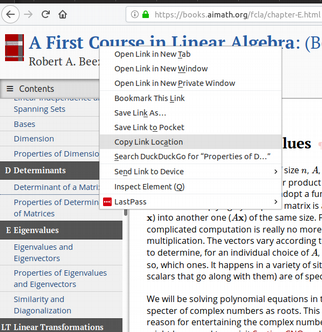
\includegraphics[width=1\linewidth]{images/section-URL.png}
\end{sbspanel}
\begin{sbscaption}{0.65}
\end{sbscaption}
\begin{sbscaption}{0.35}
\captionof{figure}{Copying URL for a subsection.\label{figure-section-url}}
\end{sbscaption}
\end{sidebyside}
\typeout{************************************************}
\typeout{Paragraphs  Index}
\typeout{************************************************}
\paragraph[{Index}]{Index}\hypertarget{paragraphs-2}{}
\begin{sidebyside}{2}{0.01}{0.01}{0.02}
\begin{sbspanel}{0.48}
\hypertarget{p-8}{}%
Instructors can add direct links to more specific items (technically any division with an @xml:id tag). An easy way to find the relevant link is to locate the item in the index of each textbook. Clicking the item in the index will open a small box (a "knowl") and display the definition of the item. Each box contains an "In Context" link in the lower right. Instructors can right-click this link to copy the URL.%
\end{sbspanel}
\begin{sbspanel}{0.48}
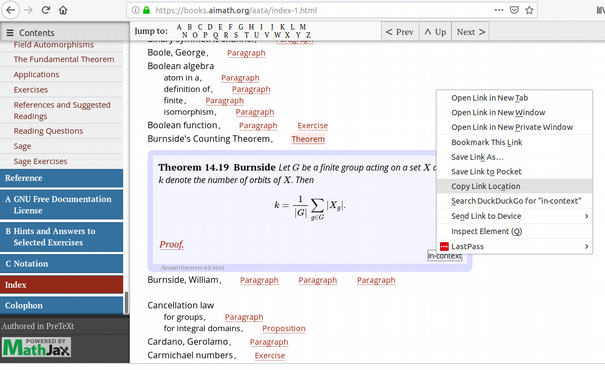
\includegraphics[width=1\linewidth]{images/knowl-URL.png}
\end{sbspanel}
\begin{sbscaption}{0.48}
\end{sbscaption}
\begin{sbscaption}{0.48}
\captionof{figure}{Copying URL for an index item.\label{figure-knowl-url}}
\end{sbscaption}
\end{sidebyside}
\typeout{************************************************}
\typeout{Paragraphs  Others}
\typeout{************************************************}
\paragraph[{Others}]{Others}\hypertarget{paragraphs-3}{}
\hypertarget{p-9}{}%
Many divisions in a PreTeXt textbook are decorated with a faint paragraph sign ¶ (known as a "pilcrow"). These pilcrows represent links which center the browser at that division. Once clicked, the URL displayed in the browser's address bar can be copied and used in other documents.%
\typeout{************************************************}
\typeout{Subsection 1.2 Sage Advice}
\typeout{************************************************}
\subsection[{Sage Advice}]{Sage Advice}\label{subsection-sage-cells}
\hypertarget{p-10}{}%
\href{https://www.sagemath.org/}{Sage} is an open source language for doing mathematics. It is designed to replicate the functionality of popular computer algebra systems (\emph{Mathematica}, MAPLE, etc.) in a unified, open source environment. It is free and may be downloaded and run locally on a user's personal computer. Many PreTeXt authors deploy what are known as Sage Cells like those seen above. These are one-off computing environments in which snippets of code can be executed and displayed in a browser without need for any installation of software on the user's part. The code can be altered in any way the user sees fit, and the original content can be restored by reloading the page.%
\par
\hypertarget{p-11}{}%
Seriously, these things are great.%
\begin{sageinput}
A = matrix(4,5, srange(20))
A.rref()
\end{sageinput}
\begin{sageoutput}
[ 1  0 -1 -2 -3]
[ 0  1  2  3  4]
[ 0  0  0  0  0]
[ 0  0  0  0  0]
\end{sageoutput}
\begin{sageinput}
var("x,y")
plot3d(x^2+y^2,(x,0,2),(y,0,2))
\end{sageinput}
\hypertarget{p-12}{}%
For those who wish to demonstrate or experiment further with Sage, AIM also hosts the the \href{https://utmost.aimath.org/sage-cell-repository/}{Sage Cell Repository}. One can compute directly on the home page or explore the \href{http://utmost-sage-cell.org/topics}{dozens of examples} compiled in the wiki.%
\typeout{************************************************}
\typeout{Section 2 Textbook-Specific Information}
\typeout{************************************************}
\section[{Textbook-Specific Information}]{Textbook-Specific Information}\label{section-textbook-specifics}
\hypertarget{p-13}{}%
This section provides specific information and author-recommendations for adopters of the specific textbooks in the project.%
\typeout{************************************************}
\typeout{Subsection 2.1 Abstract Algebra: Theory and Applications}
\typeout{************************************************}
\subsection[{Abstract Algebra: Theory and Applications}]{Abstract Algebra: Theory and Applications}\label{subsection-aata}
\leavevmode%
\begin{sidebyside}{2}{0.0125}{0.0125}{0.025}
\begin{sbspanel}{0.25}

\includegraphics[width=1\linewidth]{images/cover-aata.png}
\end{sbspanel}
\begin{sbspanel}{0.7}
\hypertarget{p-14}{}%
This page provides complementary information for participants of the UTMOST project. Because this is a \href{https://books.aimath.org/aata/index.html}{hosted version for the UTMOST project}, it is important for you to be aware of a few additional features of the textbook.%
\end{sbspanel}
\end{sidebyside}
\typeout{************************************************}
\typeout{Paragraphs  Syllabus}
\typeout{************************************************}
\paragraph[{Syllabus}]{Syllabus}\hypertarget{paragraphs-4}{}
\hypertarget{p-15}{}%
Be selective in what you cover in your course. This includes the sections of the textbook as well as the Sage exercises. You can use the chapter diagram that is presented in the \href{https://books.aimath.org/aata/preface-1.html}{Preface} to make decisions about what to include or exclude.%
\typeout{************************************************}
\typeout{Paragraphs  Sage}
\typeout{************************************************}
\paragraph[{Sage}]{Sage}\hypertarget{paragraphs-5}{}
\hypertarget{p-16}{}%
The HTML format of the textbook takes advantage of the Sage programming language. Get acquainted with \href{https://books.aimath.org/aata/sets-sage.html}{how this textbook uses Sage} to learn more about it. Instructors can either assign this section to the students, or spend some time in class to illustrate how Sage works. The cells will take Python commands.%
\par
\hypertarget{p-17}{}%
Each section of the HTML format of textbook contains Sage Exercises; they vary in complexity. The goal of these exercises is to get users to use technology to explore structures and make conjectures that would be very difficult to do by hand computation.%
\par
\hypertarget{p-18}{}%
For example, the \href{https://books.aimath.org/aata/cyclic-sage-exercises.html}{Sage Exercises in Cyclic Groups} were written to help readers explore the cyclic patterns of the group of units mod \(n\), \(U(n)\), which is sometimes cyclic, sometimes not. By using Sage, users can easily test whether or not the \(U(n)\) is cyclic for large values of \(n\) and then make a conjecture about what the general case should be.%
\par
\hypertarget{p-19}{}%
Sage can be used by typing a command line in a terminal window, in a Sage worksheet, and in the Jupyter notebook; however, the most friendly way to learn Sage is to use the Sage cell server.  The Sage cell server allows Sage to be embedded in any web page.  Users can modify and execute the Sage code.  If the edited code results in disaster, one only needs to reload the web page to restore the original code.  See the \href{http://utmost-sage-cell.org}{Sage Cell Repository} for more information.%
\typeout{************************************************}
\typeout{Paragraphs  Reference}
\typeout{************************************************}
\paragraph[{Reference}]{Reference}\hypertarget{paragraphs-reference}{}
\hypertarget{p-20}{}%
This textbook includes a \href{https://books.aimath.org/aata/backmatter.html}{Reference} section that includes appendices and the index. Of particular note is the Notation appendix which includes a list of symbolic notation and links to their occurrences in the text.%
\typeout{************************************************}
\typeout{Subsection 2.2 Active Calculus}
\typeout{************************************************}
\subsection[{Active Calculus}]{Active Calculus}\label{subsection-ac}
\leavevmode%
\begin{sidebyside}{2}{0.0125}{0.0125}{0.025}
\begin{sbspanel}{0.25}
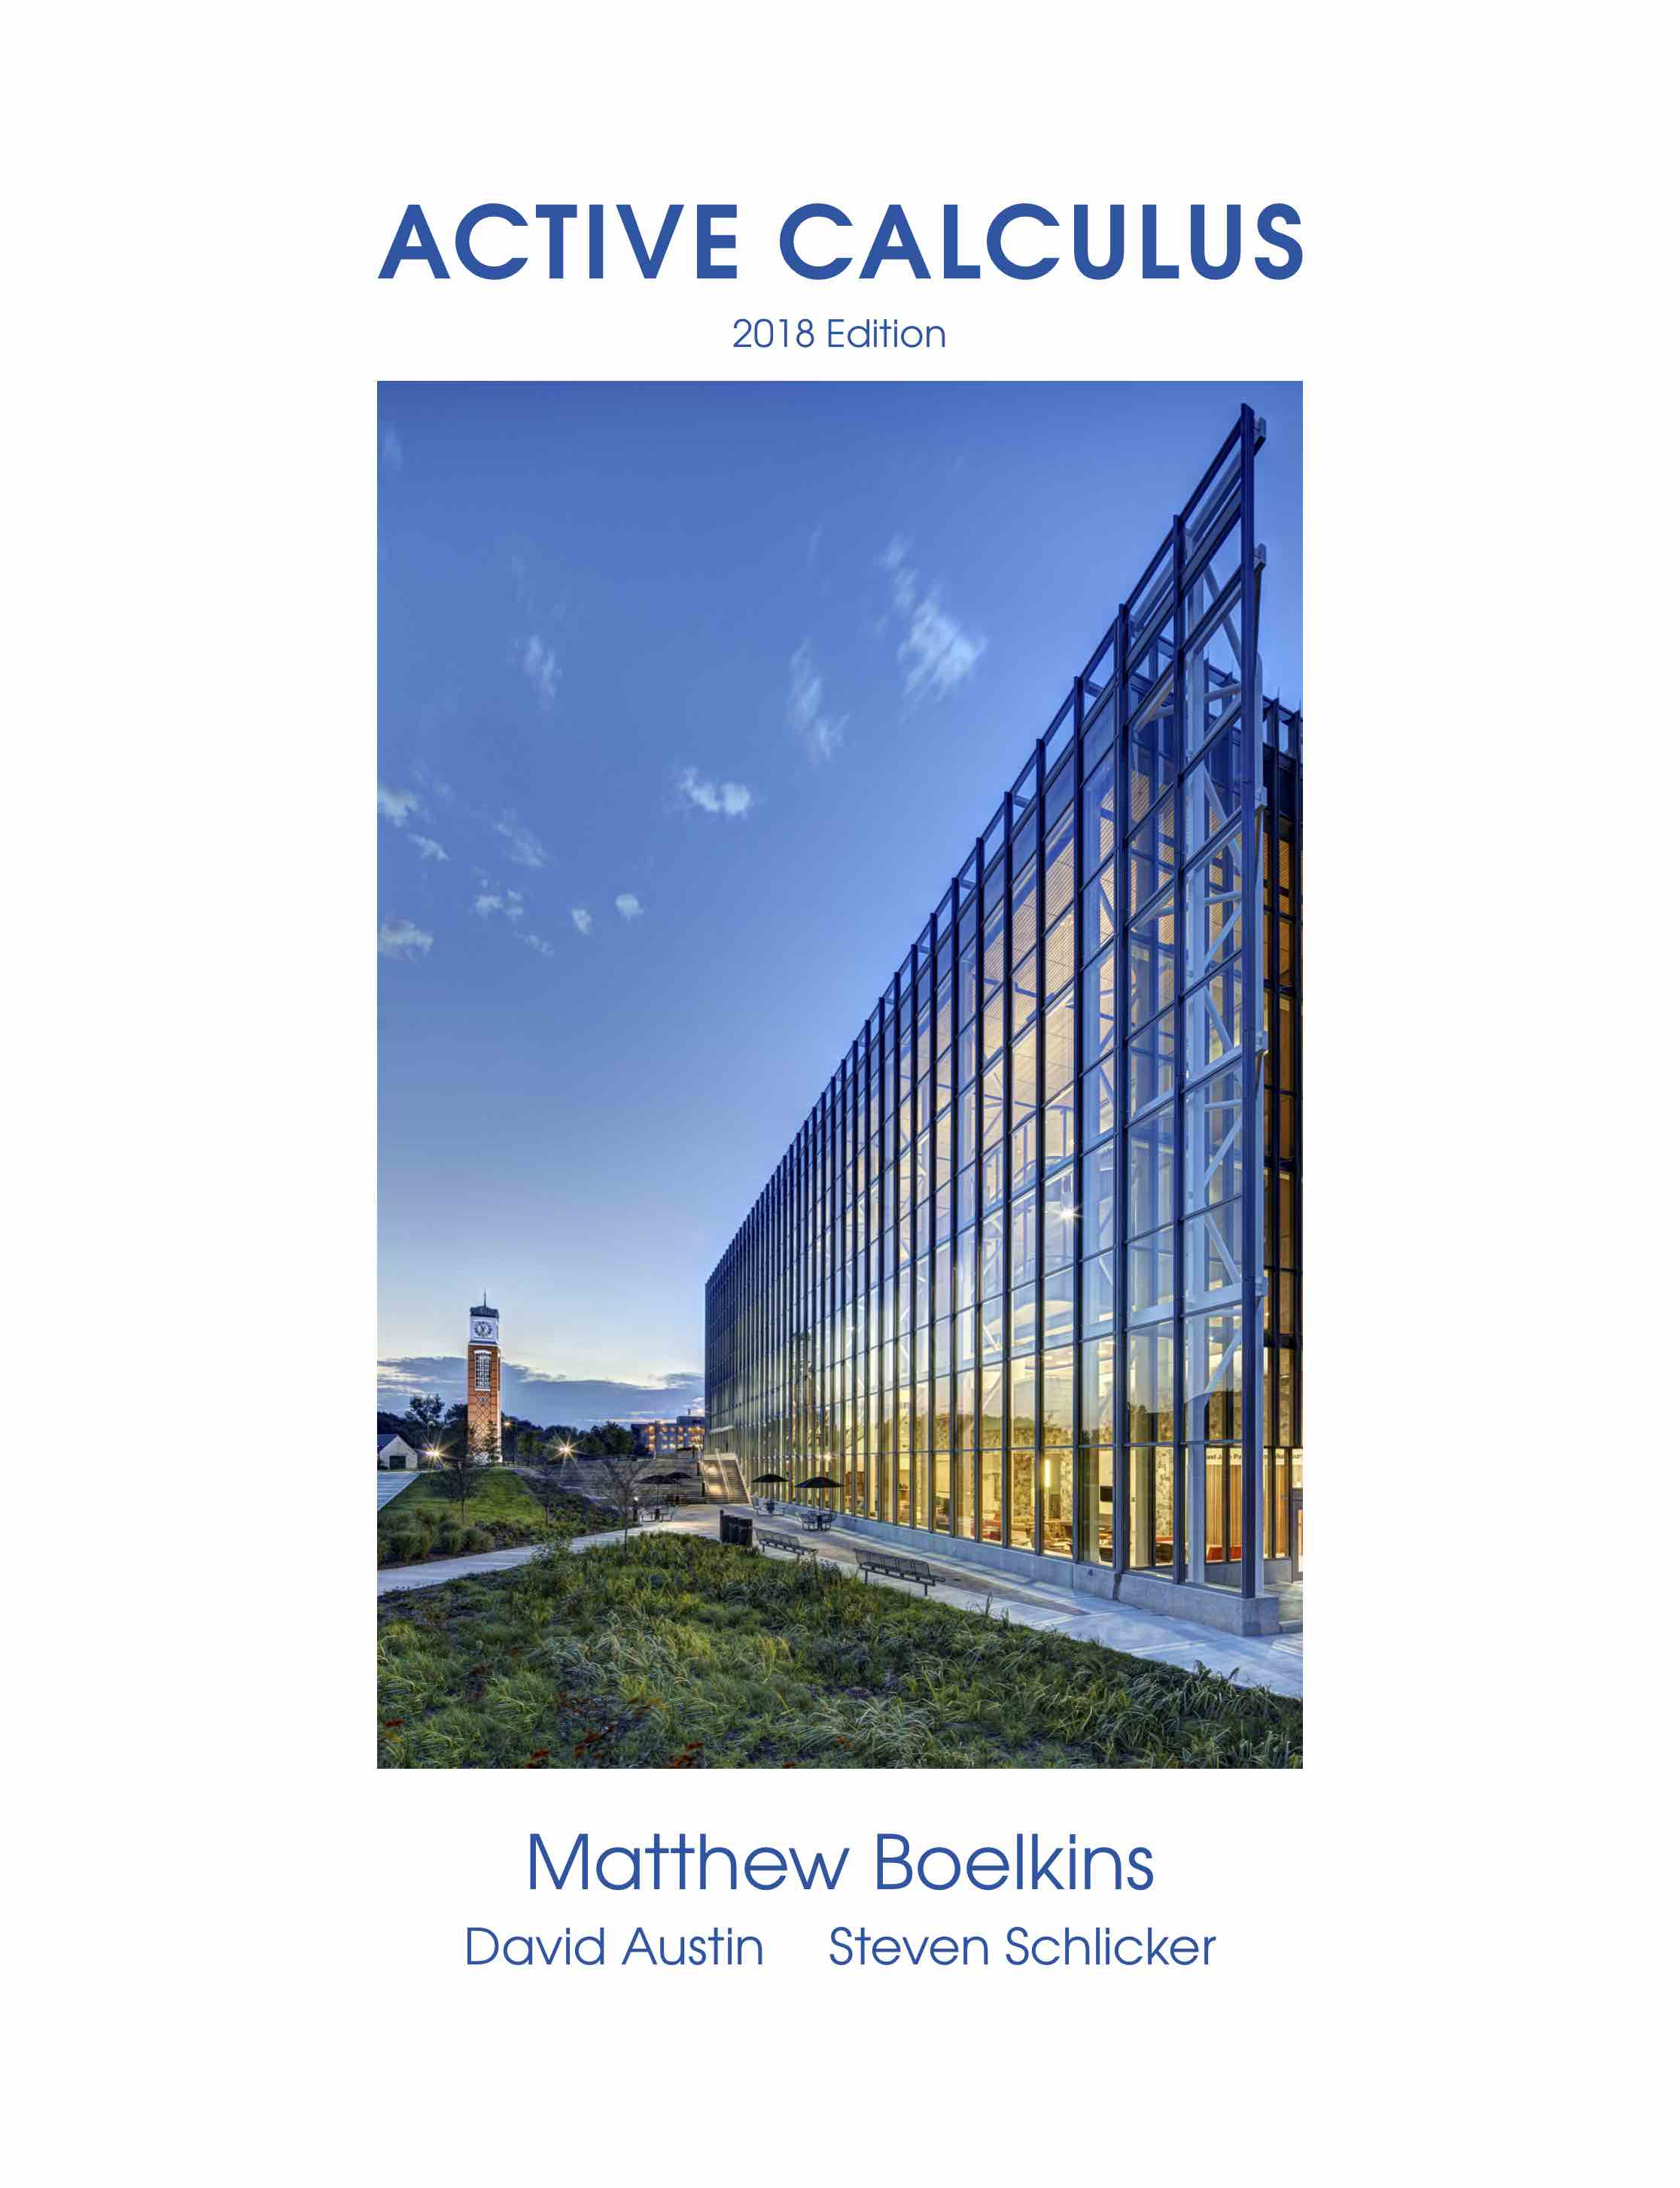
\includegraphics[width=1\linewidth]{images/cover-ac.jpg}
\end{sbspanel}
\begin{sbspanel}{0.7}
\hypertarget{p-21}{}%
This page provides complementary information to the section \href{https://books.aimath.org/ac/preface-3.html}{Features of the Text}. Because this is a hosted version for the UTMOST project, it is important for you to be aware of a few additional features of the textbook. In this section we highlight four features of this textbook that users need to be aware of for course and lesson planning: the Preview Activities, the Class Activities, WeBWorK, and Solutions.%
\end{sbspanel}
\end{sidebyside}
\typeout{************************************************}
\typeout{Paragraphs  Preview Activities}
\typeout{************************************************}
\paragraph[{Preview Activities}]{Preview Activities}\hypertarget{paragraphs-7}{}
\hypertarget{p-22}{}%
In addition to the Reading Questions, each section begins with a Preview Activity, meant to be an accessible introduction to new ideas that rely largely on knowledge that students already have. Most Preview Activities can be completed in 15\textendash{}20 minutes. If students are logged in to the HTML version of the text, the Preview Activities can be completed in the HTML version and the responses reviewed by the instructor.  Instructors can incentivize the completion of the Preview Activities by asking the students to put their work on their desks for review in class.%
\typeout{************************************************}
\typeout{Paragraphs  Activities}
\typeout{************************************************}
\paragraph[{Activities}]{Activities}\hypertarget{paragraphs-8}{}
\hypertarget{p-23}{}%
Each section in the textbook has three Activities (e.g., \href{https://books.aimath.org/ac/sec-1-3-derivative-pt.html\#Mtw}{Activity 1.3.2}) that are designed for being done in class by students. There is a PDF Activities Workbook that can be printed so students can use it to work on it in class.%
\par
\hypertarget{p-24}{}%
Students using the HTML version of the textbook can revise the responses they provide to the Preview Activity questions before they submit them. Once they are submitted, the instructor can immediately see the responses when logged into their instructor account.%
\typeout{************************************************}
\typeout{Paragraphs  WeBWorK}
\typeout{************************************************}
\paragraph[{WeBWorK}]{WeBWorK}\hypertarget{paragraphs-9}{}
\hypertarget{p-25}{}%
Almost every Exercises section of the UTMOST HTML format of the textbook includes anonymous WeBWorK exercises that students can complete and receive immediate feedback with unlimited attempts without penalty ("anonymous" here means students' work is not recorded anywhere). The WeBWorK exercises are intended to be more routine than the following non-WeBWorK exercises.%
\typeout{************************************************}
\typeout{Paragraphs  Solutions}
\typeout{************************************************}
\paragraph[{Solutions}]{Solutions}\hypertarget{paragraphs-10}{}
\hypertarget{p-26}{}%
This textbook includes an instructor's solution manual with answers and solutions to each Activity and non-WeBWorK exercise in the text. The answers are available in the publicly posted electronic versions (both HTML and PDF).  The solutions manual is only available to instructors by direct request by email to the author (boelkinm at gvsu dot edu).%
\typeout{************************************************}
\typeout{Subsection 2.3 A First Course in Linear Algebra}
\typeout{************************************************}
\subsection[{A First Course in Linear Algebra}]{A First Course in Linear Algebra}\label{subsection-fcla}
\leavevmode%
\begin{sidebyside}{2}{0.0125}{0.0125}{0.025}
\begin{sbspanel}{0.25}
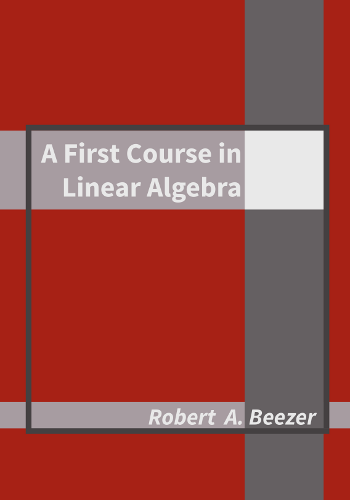
\includegraphics[width=1\linewidth]{images/cover-fcla.png}
\end{sbspanel}
\begin{sbspanel}{0.7}
\hypertarget{p-27}{}%
This page provides complementary information to the section "How to Use this Book" in the Preface of the textbook. %
\end{sbspanel}
\end{sidebyside}
\typeout{************************************************}
\typeout{Paragraphs  Topic Order}
\typeout{************************************************}
\paragraph[{Topic Order}]{Topic Order}\hypertarget{paragraphs-11}{}
\hypertarget{p-28}{}%
It is not recommended to change the order of the sections in the textbook because each chapter builds upon what has been done before.%
\typeout{************************************************}
\typeout{Paragraphs  Acronyms}
\typeout{************************************************}
\paragraph[{Acronyms}]{Acronyms}\hypertarget{paragraphs-12}{}
\hypertarget{p-29}{}%
This textbook does not use numbering system for the sections as other textbooks. The author uses acronyms to refer to each section, as they encode information about that content, that is more useful than “Theorem 5.1 is.” The best way to handle them is to use them in class continuously. Students do not have to memorize them. It is sufficient  that they can recall what theorem they may need to use. Every chapter has annotated acronyms for definitions and theorems that remind readers the importance of each of them. Although students get anxious about the many acronyms, it is not such a big deal.%
\par
\hypertarget{p-30}{}%
Of great help to both instructors and students is the \href{https://books.aimath.org/fcla/reference.html}{Reference} chapter. It is organized by the major sections of the textbook. Each section contains all the symbols and terminology used in that section, with a knowl that provides its definition and an "in context" link. Each of these sections is searchable.%
\typeout{************************************************}
\typeout{Paragraphs  Exercises}
\typeout{************************************************}
\paragraph[{Exercises}]{Exercises}\hypertarget{paragraphs-13}{}
\hypertarget{p-31}{}%
This textbook has three categories of exercises: computational (labeled as C), conceptual (labeled as M), and theoretical (labeled as T). The author has a particular numbering system that does not mean much. It allows adding and changing problems as needed.%
\typeout{************************************************}
\typeout{Paragraphs  Proof Techniques}
\typeout{************************************************}
\paragraph[{Proof Techniques}]{Proof Techniques}\hypertarget{paragraphs-14}{}
\hypertarget{p-32}{}%
The textbook contains a chapter on \href{https://books.aimath.org/fcla/appendix-PT.html}{Proof Techniques} that has been included to support students as they build their proving skills. Instructors can remind the students of the techniques that are available and explained in this chapter.%
\typeout{************************************************}
\typeout{Paragraphs  Archetypes}
\typeout{************************************************}
\paragraph[{Archetypes}]{Archetypes}\hypertarget{paragraphs-15}{}
\hypertarget{p-33}{}%
The textbook works with examples called \href{https://books.aimath.org/fcla/appendix-A.html}{Archetypes}, labeled with a letter, and ordered alphabetically. The Archetypes provide a range of examples that fit specific properties. They are included to serve as illustrations for how properties work or fail. They can be used to test conjectures. The students can be encouraged to check them whenever they are learning new material. The archetypes include the relevant theorems.%
\typeout{************************************************}
\typeout{Paragraphs  Sage}
\typeout{************************************************}
\paragraph[{Sage}]{Sage}\hypertarget{paragraphs-16}{}
\hypertarget{p-34}{}%
The textbook makes heavy use of Sage cells (there are 96 vignettes with Sage cells, a list of which can be found here \href{https://books.aimath.org/fcla/appendix-SL.html}{Sage}). These are intended to help students learn to use Sage to do linear algebra and to learn how to do linear algebra by using computational examples. There is a separate \href{https://github.com/rbeezer/sla}{GitHub repository} that contains 17 Sage worksheets that instructors can use in class (in several output formats, including Jupyter, PDF, etc.).  They are "incomplete" and meant to be filled in during class. For some examples, a random elements are generated; in others, a carefully constructed example is explicitly defined. There is a \href{https://github.com/rbeezer/sla/blob/master/worksheets/overview.pdf}{master document} with a short description and expected duration (usually between 5 and 20 minutes) for each. Instructors can do them in class. they can see many different examples in class.%
\typeout{************************************************}
\typeout{Section 3 UTMOST-Specific Information}
\typeout{************************************************}
\section[{UTMOST-Specific Information}]{UTMOST-Specific Information}\label{section-utmost-specifics}
\hypertarget{p-35}{}%
This guide is intended for instructors at test sites participating in the UTMOST project (hence the use of second person). It may not be relevant to a general audience.%
\typeout{************************************************}
\typeout{Subsection 3.1 Version}
\typeout{************************************************}
\subsection[{Version}]{Version}\label{subsection-version}
\hypertarget{p-36}{}%
Being open-source textbooks, there may be several (maybe dozens) of implementations of your textbook on the open web. It is \emph{very important} you and your students use the UTMOST-specified version of the text.%
\par
\hypertarget{p-37}{}%
Different sites have been designated to use either the HTML (online) format of the textbook or the PDF (offline or printed) format. Find the relevant links below.%
\typeout{************************************************}
\typeout{Paragraphs  HTML Format}
\typeout{************************************************}
\paragraph[{HTML Format}]{HTML Format}\hypertarget{paragraphs-17}{}
\hypertarget{p-38}{}%
\leavevmode%
\begin{itemize}[label=\textbullet]
\item{}\href{https://books.aimath.org/aata/}{Abstract Algebra: Theory and Applications}%
\item{}\href{https://books.aimath.org/ac/}{Active Calculus}%
\item{}\href{https://books.aimath.org/fcla/}{A First Course in Linear Algebra}%
\end{itemize}
%
\par
\hypertarget{p-39}{}%
You and your students will be given logins for the AIM-hosted version of your textbook. As mentioned, it is crucially important that you use and bookmark this version. The login should persist on a given device so that frequent logging in will be unnecessary.%
\typeout{************************************************}
\typeout{Paragraphs  PDF Format}
\typeout{************************************************}
\paragraph[{PDF Format}]{PDF Format}\hypertarget{paragraphs-18}{}
\hypertarget{p-40}{}%
\leavevmode%
\begin{itemize}[label=\textbullet]
\item{}\href{}{Abstract Algebra: Theory and Applications}%
\item{}\href{}{Active Calculus}%
\item{}\href{}{A First Course in Linear Algebra}%
\end{itemize}
%
\typeout{************************************************}
\typeout{Subsection 3.2 Highlighting}
\typeout{************************************************}
\subsection[{Highlighting}]{Highlighting}\label{subsection-highlighting}
\typeout{************************************************}
\typeout{Paragraphs  HTML Format}
\typeout{************************************************}
\paragraph[{HTML Format}]{HTML Format}\hypertarget{paragraphs-19}{}
\hypertarget{p-41}{}%
The hosted versions of the texbooks include a feature whereby students can highlight portions of the text and have those highlights persist across different versions. Instructors' versions makes this available as well, though when text is highlighted, they are given the choice to highlight or simply copy the text to the clipboard.%
\typeout{************************************************}
\typeout{Paragraphs  PDF Format}
\typeout{************************************************}
\paragraph[{PDF Format}]{PDF Format}\hypertarget{paragraphs-20}{}
\hypertarget{p-42}{}%
There are many ways to annotate a PDF, but such is not the goal of this document.%
\typeout{************************************************}
\typeout{Subsection 3.3 Reading Questions}
\typeout{************************************************}
\subsection[{Reading Questions}]{Reading Questions}\label{subsection-reading-questions}
\hypertarget{p-43}{}%
As you cover material in various parts of the book, it is important you assign the Reading Questions for the relevant sections. The authors have written them as a quick check on readers' comprehension after first exncountering the material of a section. These can be of great help to the researchers, the instructor, and, indeed, the students themselves.%
\par
\hypertarget{p-44}{}%
It is at the instructor's discretion exactly when and how exactly to assign these, but it is highly recommended that a small percentage of their grade depend on the completion thereof.%
\typeout{************************************************}
\typeout{Paragraphs  HTML Format}
\typeout{************************************************}
\paragraph[{HTML Format}]{HTML Format}\hypertarget{paragraphs-21}{}
\hypertarget{p-45}{}%
With the AIM-hosted versions of the textbooks, students are able to answer the reading question right in their browsers. Their answers can then be displayed in the instructor's version. Whether reading is assigned before or after material is covered in class, a quick scan of the responses can inform the instructor if some material requires further attention.%
\par
\hypertarget{p-46}{}%
Researchers will receive and analyze anonymized copies of student responses.%
\typeout{************************************************}
\typeout{Paragraphs  PDF Format}
\typeout{************************************************}
\paragraph[{PDF Format}]{PDF Format}\hypertarget{paragraphs-22}{}
\hypertarget{p-47}{}%
for the PDF versions of the textbooks are distributed separately, and can be found by (((FILL THIS IN)))%
\par
\hypertarget{p-48}{}%
You may want to set up your LMS so that students can input their responses there. Many systems (e.g., Canvas) have a "Discussions" tool in which the Reading Questions can be posted as prompts and students reply after which their peers' replies become visible.%
 `\end{document}